\chapter{Multiview Geometry and Structure from Motion}
\label{chapter:3D_multiview}

\section{Introduction}

As humans, we know how it feels to look at the world with one eye. We can easily experience this by closing one eye, or when looking at a picture. The world clearly appears to us as three-dimensional (3D), but there is something that still feels somewhat flat. 
We also know what it is to look at the world with two eyes. Objects and scenes appear and feel 3D. We sense the volume of the space. In fact, even when we look with both of our eyes at a flat surface we feel it is 3D as we can feel how far the surface is and what is its orientation. 
%But we cannot imagine what it is to look at the world with many eyes. We can try to guess it, but we will fall short just as if we were trying to guess what the world would feel like when looking at it with two eyes if we had only one eye. 
But we do not know what it is to look at the world with three or more eyes. We can try to make guesses about what new sensations we might feel, but we are likely to fall short in truly understanding how it feels to see world through many eyes.  It's like someone with one eye trying to envision seeing the world with two; we can make guesses, but our comprehension will be limited.

% We struggle to truly understand how the world appears when viewed with many eyes. It's like someone with one eye trying to envision seeing the world with two; we can make guesses, but our comprehension will be limited.

Looking at an object simultaneously with many eyes surrounding the object, we will not only feel its 3D but also its wholeness in a way hard to imagine with only two eyes. For us, only one side of the object is visible at any given time. We can turn around an object to see all of its sides, but that will not compare with the simultaneous perception of all its sides. 

Multiview geometry studies the 3D reconstruction of an object or a scene when captured from $N$ cameras (with $N>2$). 


\section{Structure from Motion}

%Walkers and body points 
% https://www.youtube.com/watch?v=1F5ICP9SYLU
%The interpretation of structure from motion by Shimon Ullman, 1979

In 1971, Gunnar Johansson created a series of beautiful videos by recording the movements of a person with a set of lights attached to few of the body joints (e.g., elbows, knees, feet, head, and hands as illustrated in \fig{\ref{fig:demos_motivation_sfm}}[b]). 

\marginnote{Gunnar Johansson was a Swedish psychologist working on gestalt laws of motion perception. He introduced the term of {\bf biological motion}\index{Biological motion} to describe the typical motion of biological organisms.}

Johansson \cite{Johansson1973} demonstrated that by watching the motion of only a few of those points, no more than 12, it was possible to clearly recognize the person actions. By showing only moving points, Johansson dissociated the perception of form/shape from the motion pattern. Johansson's videos were very surprising at the time and researchers were stunned by how easy was to recognize many types of actions from just a few moving points. 
Since then, Johansson's early demonstrations have been used to argue about the importance of reliably tracking a few points over time. 







%Point-light walkers are videos showing only a few points (\fig{\ref{fig:demos_motivation_sfm}}{b}) attached at key locations in the body of a person (e.g., elbows, knees, feet, head, hands as illustated in \fig{\ref{fig:demos_motivation_sfm}}{b}). 

%The videos demostrated that simply watching those keypoints moving was enough to understand the actions executed by the person.  

One major advance that allowed writing a mathematical formulation of the problem of structure from motion (SFM) was the {\bf rigidity assumption}\index{Rigidity assumption} introduced by Shimon Ullman in 1979 \cite{Ullman1979} where he writes: ``Any set of elements undergoing a two dimensional transformation which has a unique interpretation as a rigid body moving in space should be interpreted as such a body in motion.'' Since then, the 3D reconstruction of rigid objects from camera motion has been a rich area of work. Most of the works start by representing the sequence using as input the temporal trajectories of a sparse set of points ({\bf sparse SFM}). \Fig{\ref{fig:demos_motivation_sfm}}{a} shows one frame from the nested cylinders sequence. In this sequence, there are a set of points placed on the surface of two nested cylinders. The cylinders are rotating. When viewing the sequence it is easy to see both cylinders, even though when seeing any single frame (as shown in \fig{\ref{fig:demos_motivation_sfm}}[a]) it is hard to see the cylinders or even to say which points are attached to the same surface. 

%The problem of structure from motion (SFM) was first explicitly formulated in computer vision by Shimon Ullman in 1979 \cite{Ullman1979} where he writes: ``{\em Any set of elements undergoing a two dimensional transformation which has a unique interpretation as a rigid body moving in space should be interpreted as such a body in motion}''. Since then, the 3D reconstruction of rigid objects from camera motion has been a rich area of work and most of the works have started by using as input the temporal trajectories of a sparse set of points. \Fig{\ref{fig:demos_motivation_sfm}}{a} shows one frame from the nested cylinders sequence. In this sequence, there are a set of points placed on the surface of two nested cylinders. The cylinders are rotating. When viewing the sequence, it is easy to see both cylinders even though when seeing any single frame it is hard to see the cylinders or even to say which points are attached to the same surface. 

\begin{figure}
\centerline{
\includegraphics[width=.7\linewidth]{figures/sfm/demos_motivation.eps}
} 
\caption{Early illustrations on the perceptual power of motion. (a) Nested cylinders by Shimon Ullman, 1979, illustrated how rigid motion elicits a strong 3D interpretation. (b) One frame from the point-light walker by Gunnar Johansson, as an early illustration of biological motion perception from few moving keypoints.}
\label{fig:demos_motivation_sfm}
\end{figure}


One of the first algorithms for structure from motion for rigid bodies was introduced by Tomasi and Kanade \cite{Tomasi92}. For simplicity, their approach assumed parallel projection (orthographic camera) instead of perspective projection. The algorithm took as input a video sequence captured by a moving camera looking at a static scene. The video was first processed by extracting keypoints and tracking them over time. The input to the reconstruction algorithm was the keypoint trajectories and the output was the 3D locations of those points with respect to a reference world-coordinate system (usually defined by the first frame in the video). 
 The model introduced by Tomasi and Kanade was later extended by Sturm and Triggs \cite{Sturm1996} to handle perspective projection.

%Tomasi and T. Kanade. Shape and motion from image streams under orthography: a factorization method. International Journal of Computer Vision, 9(2):137–154, 1992. 



%F. Sturm and B. Triggs. A factorization based algorithm for multi image projective structure and motion. In European Conference on Computer Vision (ECCV), pages 709–720, 1996

One of the key problems in SFM is to find correspondences across multiple images. Finding image correspondences is a topic that we have already mentioned in multiple places (e.g., \chap{\ref{chap:stereo_vision}} and \ref{chapter:homography}) and that will be mentioned again (\chap{\ref{chap:optical_flow_estimation}}).

SIFT \cite{Lowe04} made image matching more reliable and structure from motion started to work much better under difficult conditions such as where views are captured by cameras at very different locations, which is a more difficult image matching than when the views are frames from one sequence.   


The task of SFM became more general, and instead of focusing on one moving camera, SFM was applied to the problem of reconstructing the 3D scene even from multiple images taken by different cameras and making no assumption about the placement of the cameras.  The work by Snavely et al. \cite{Snavely2006} was one of the first to produce spectacular registrations and camera pose estimates of images taken with many different cameras. They showed how one could reconstruct famous buildings from pictures taken by tourists. 

In the last decade, deep learning now provides a more robust set of features for finding image correspondences, which is one of the key elements of the SFM algorithms.


%The task in structure from motion is, given a collection of $M$ images of a scene, recover the 3D structure of the scene and the location of the camera for each image. 

\section{Sparse SFM}

Let's start defining the notation and the formulation of the problem we want to solve; given a set of $M$ images with overlapping content, we want to recover the 3D structure of the scene and the location of the camera for each image. Figures \ref{fig:sfm:sugar} and \ref{fig:sfm:palma} show two examples of sets of images. \Fig{\ref{fig:sfm:sugar}} shows 12 images of an object taken by a camera moving around the object. \Fig{\ref{fig:sfm:palma}} shows eight images taken inside a plaza. Both sets of images represent very different scenarios that will be reconstructed with the same set of techniques.


\begin{figure}[t]
\centerline{
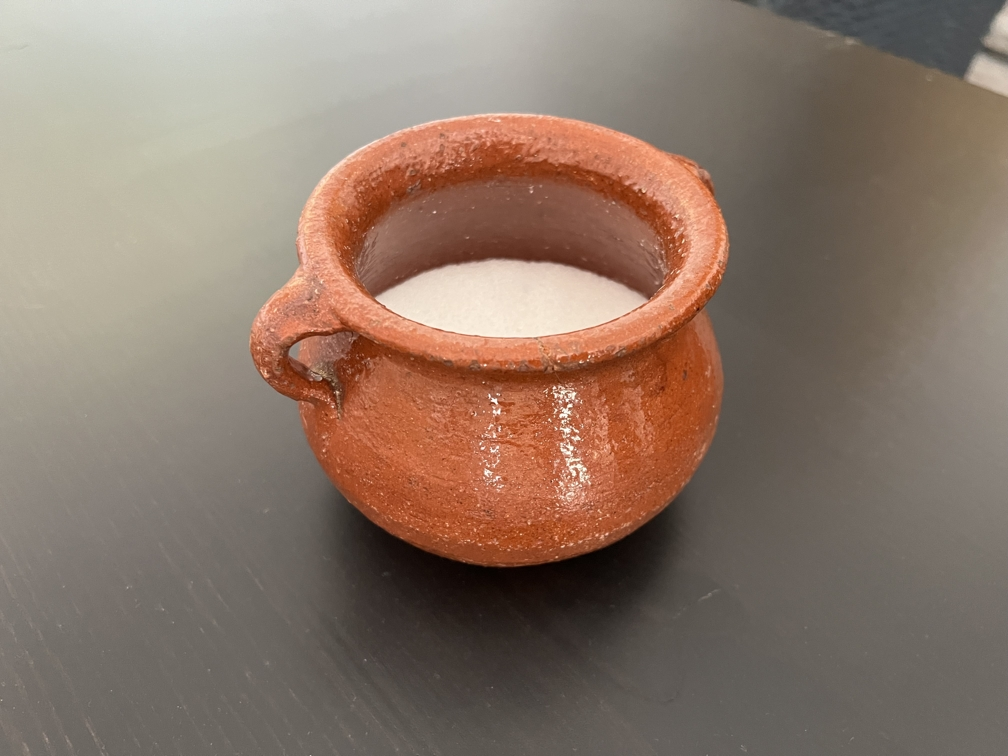
\includegraphics[width=.24\linewidth]{figures/sfm/sugar/IMG_1489.jpeg}
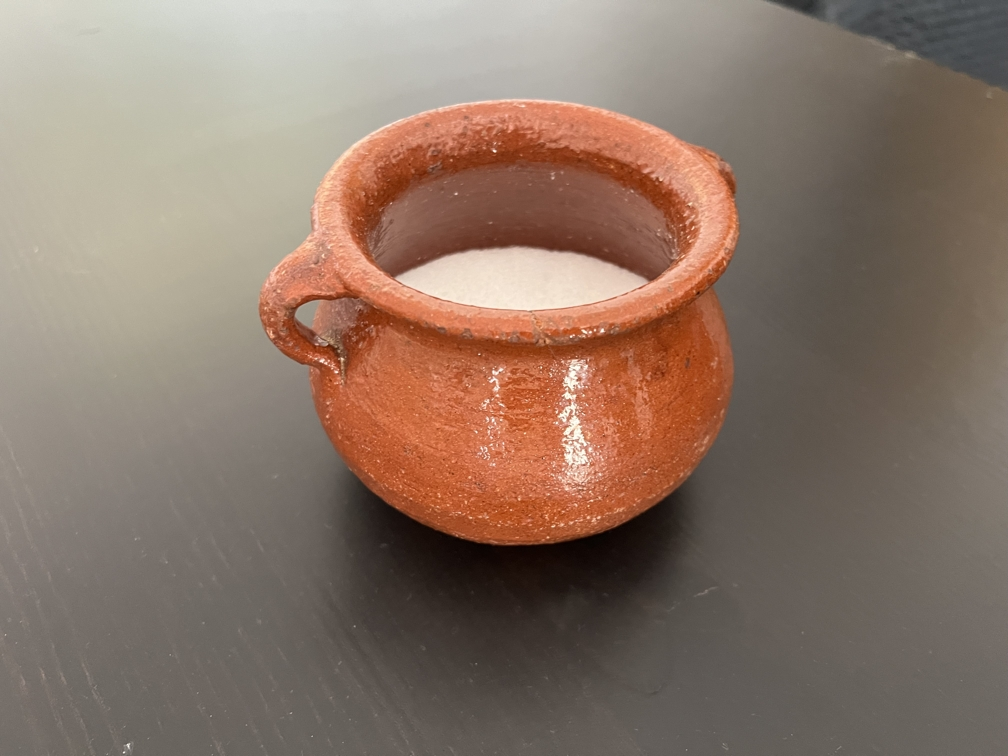
\includegraphics[width=.24\linewidth]{figures/sfm/sugar/IMG_1490.jpeg}
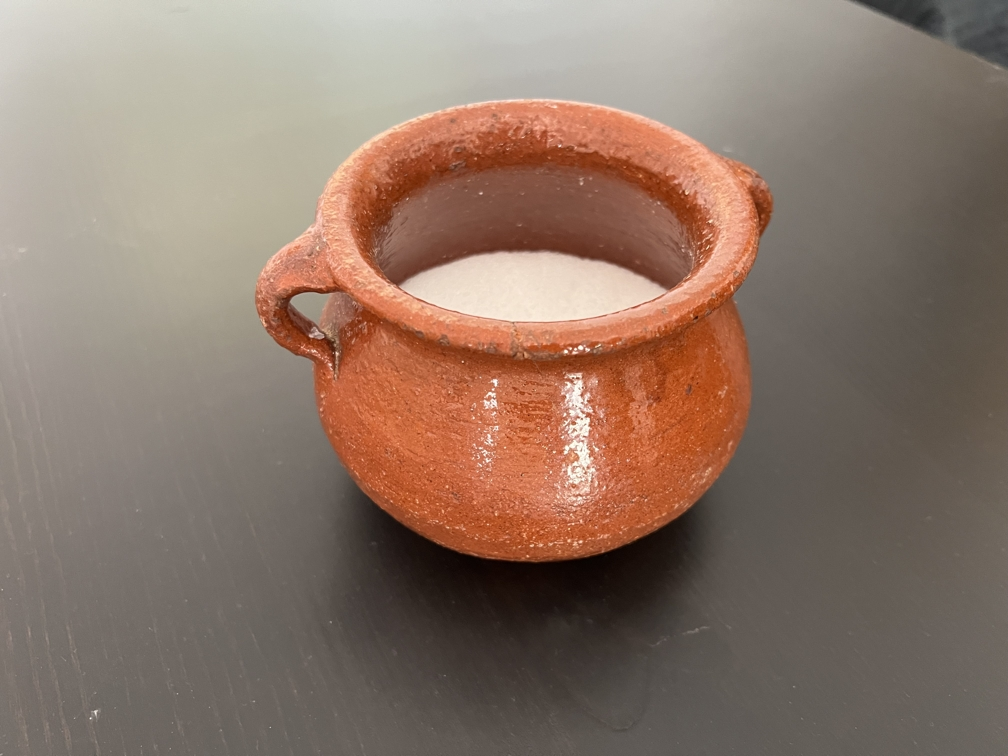
\includegraphics[width=.24\linewidth]{figures/sfm/sugar/IMG_1491.jpeg}
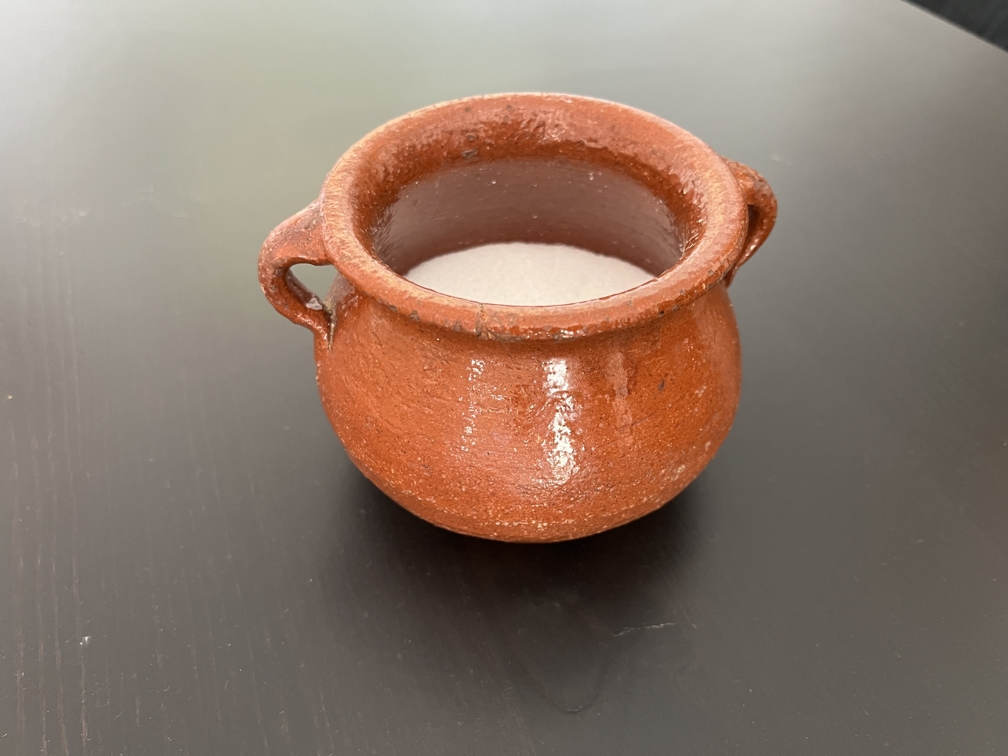
\includegraphics[width=.24\linewidth]{figures/sfm/sugar/IMG_1492.jpeg}
} 
\centerline{
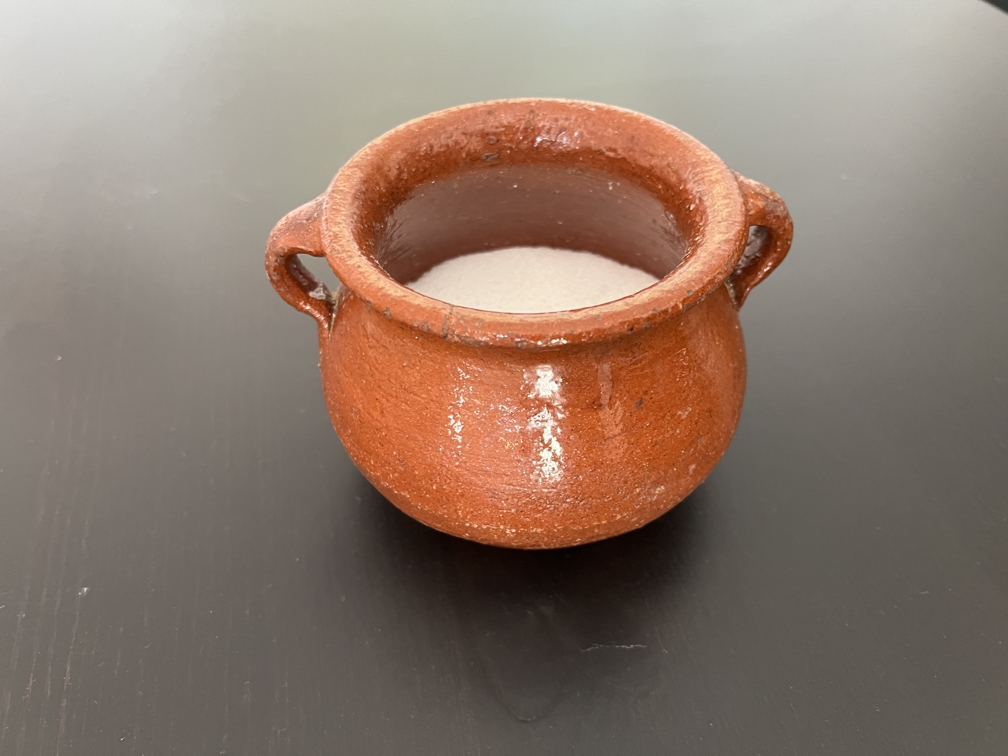
\includegraphics[width=.24\linewidth]{figures/sfm/sugar/IMG_1493.jpeg}
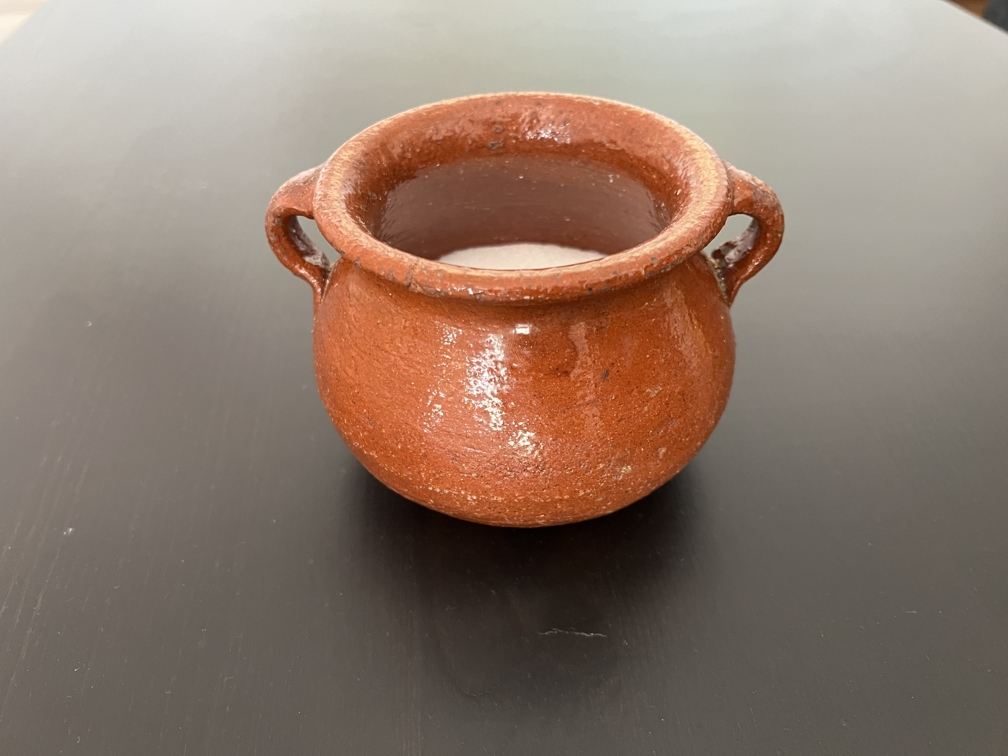
\includegraphics[width=.24\linewidth]{figures/sfm/sugar/IMG_1494.jpeg}
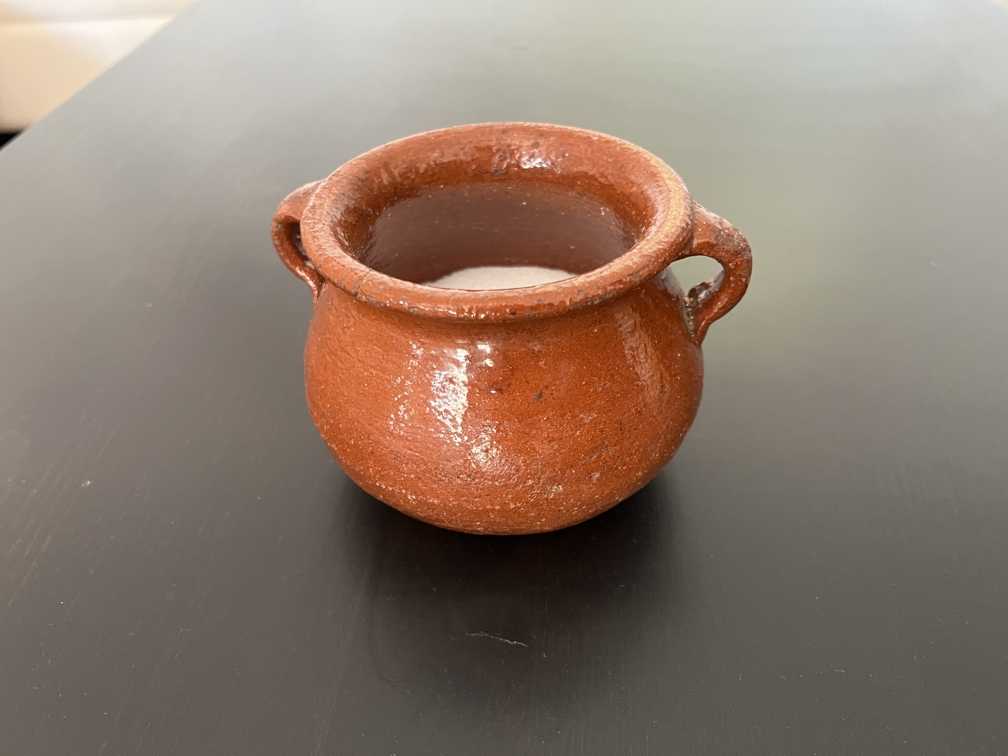
\includegraphics[width=.24\linewidth]{figures/sfm/sugar/IMG_1495.jpeg}
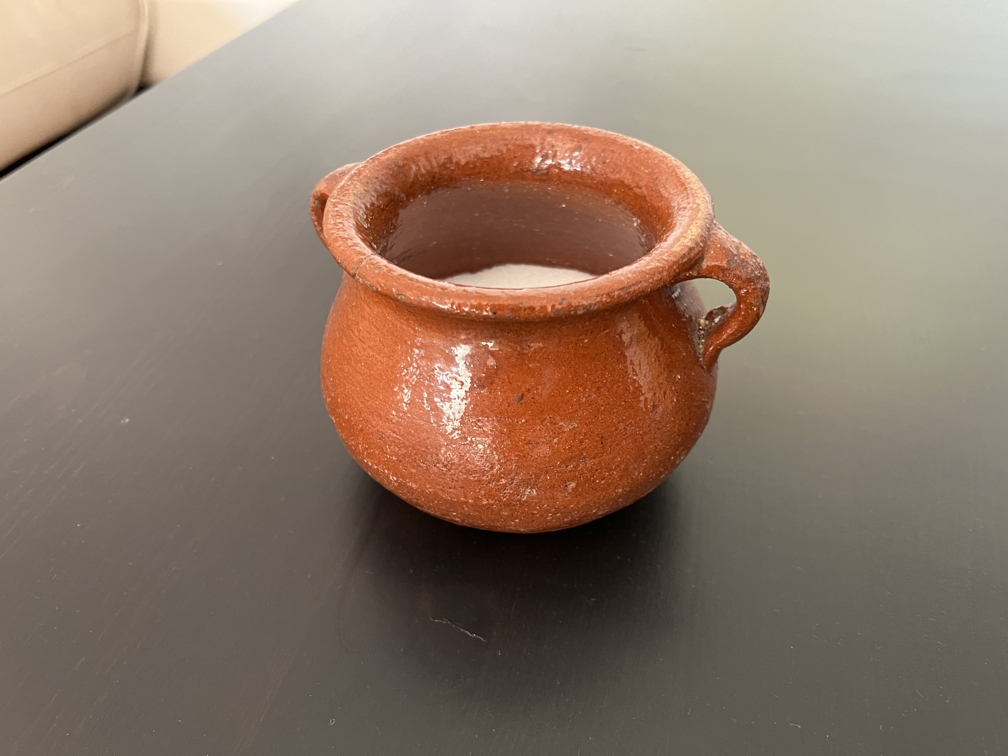
\includegraphics[width=.24\linewidth]{figures/sfm/sugar/IMG_1496.jpeg}
} 
\centerline{
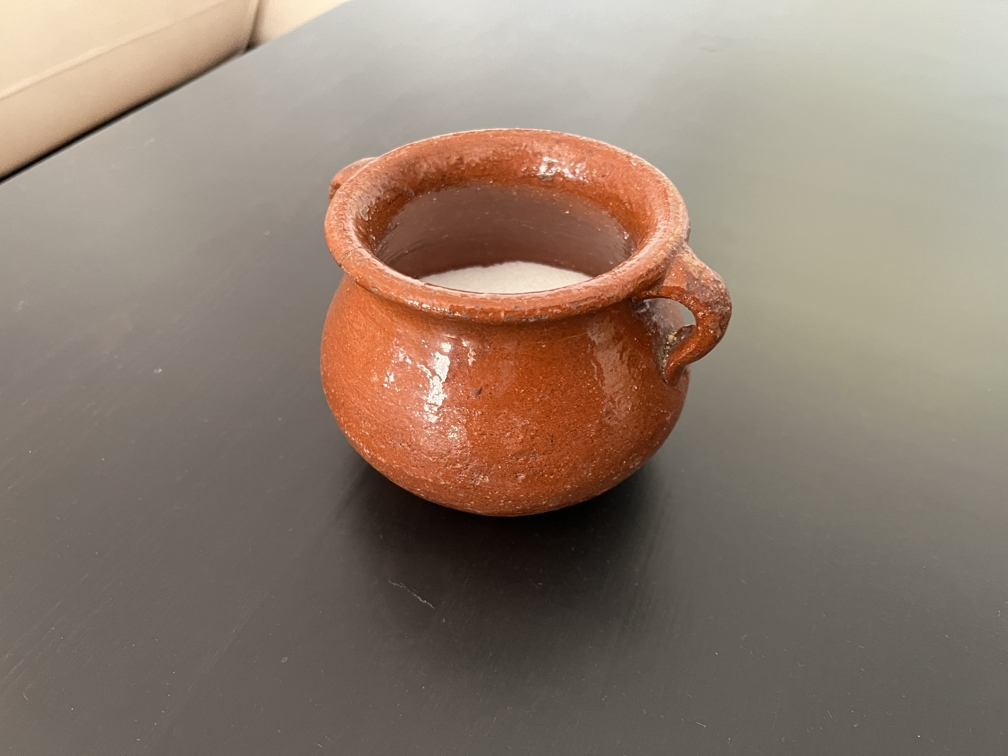
\includegraphics[width=.24\linewidth]{figures/sfm/sugar/IMG_1497.jpeg}
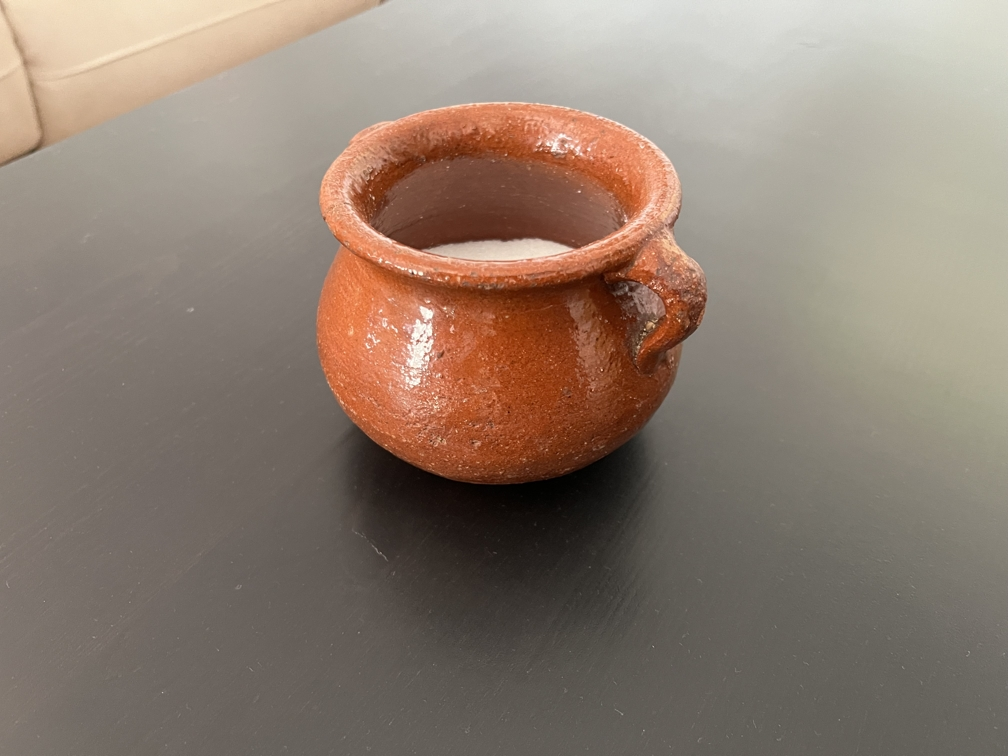
\includegraphics[width=.24\linewidth]{figures/sfm/sugar/IMG_1498.jpeg}
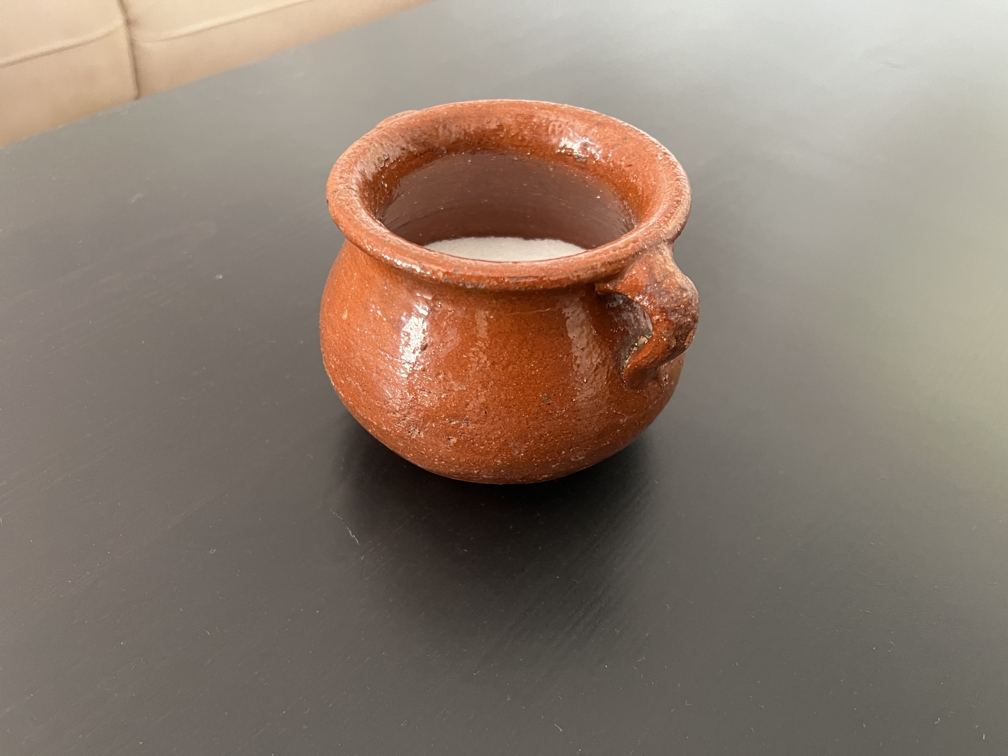
\includegraphics[width=.24\linewidth]{figures/sfm/sugar/IMG_1499.jpeg}
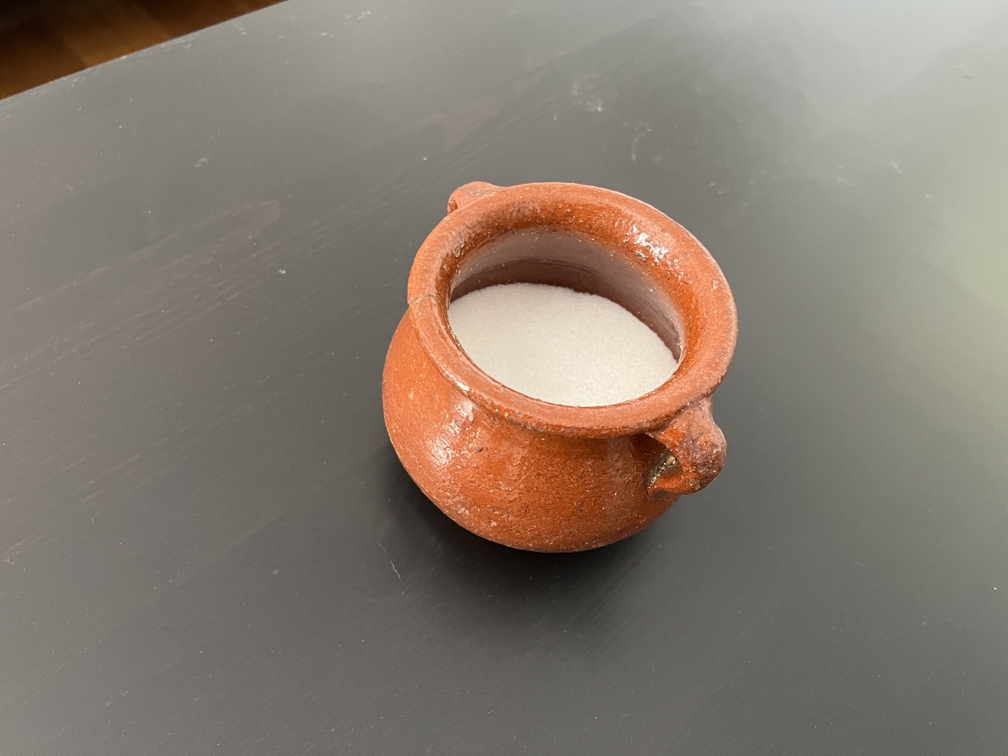
\includegraphics[width=.24\linewidth]{figures/sfm/sugar/IMG_1500.jpeg}
} 
\caption{Twelve viewpoints of a sugar bowl we had at home. Although it is not a fancy object, it is useful to start with a simple shape to check what happens on every step. The bowl has a rough texture that might also allow for enough keypoints to be present along its surface. The images have $3,024 \times 4,032$ pixels.}
\label{fig:sfm:sugar}
\end{figure}


\begin{figure}[t]
\centerline{
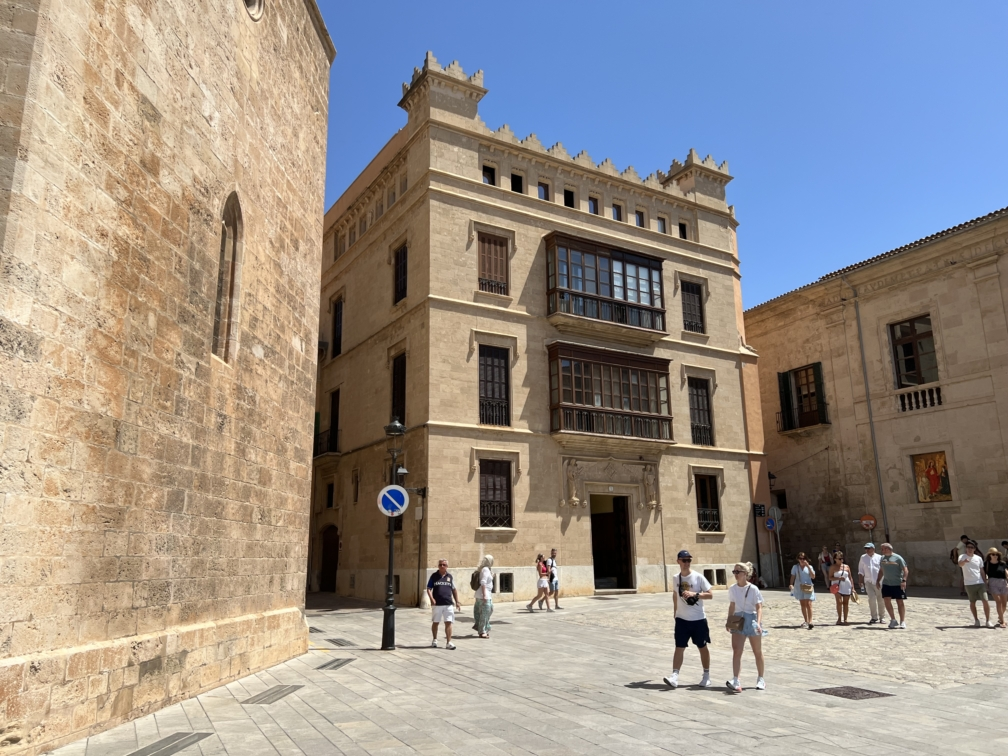
\includegraphics[width=.24\linewidth]{figures/sfm/palma/IMG_1643.jpeg}
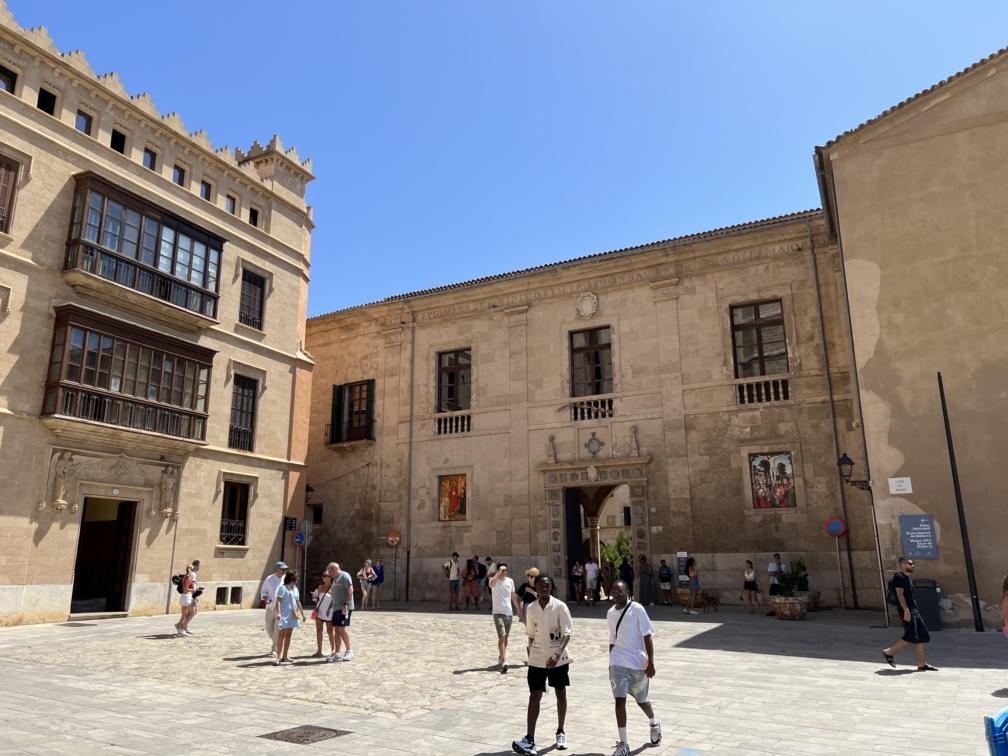
\includegraphics[width=.24\linewidth]{figures/sfm/palma/IMG_1644.jpeg}
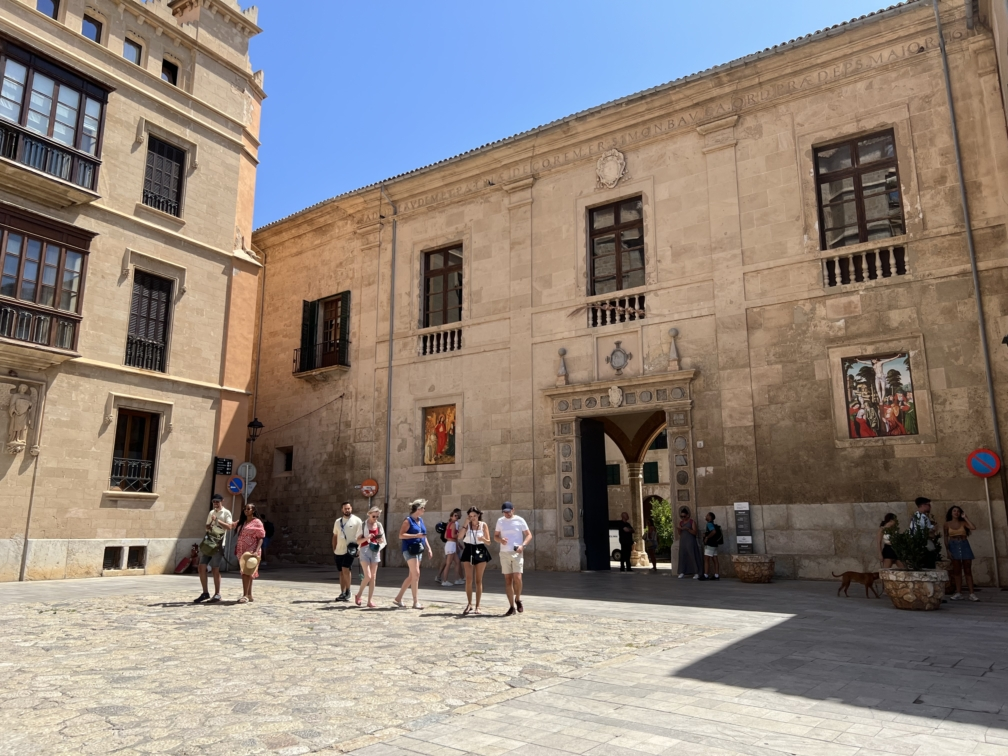
\includegraphics[width=.24\linewidth]{figures/sfm/palma/IMG_1646.jpeg}
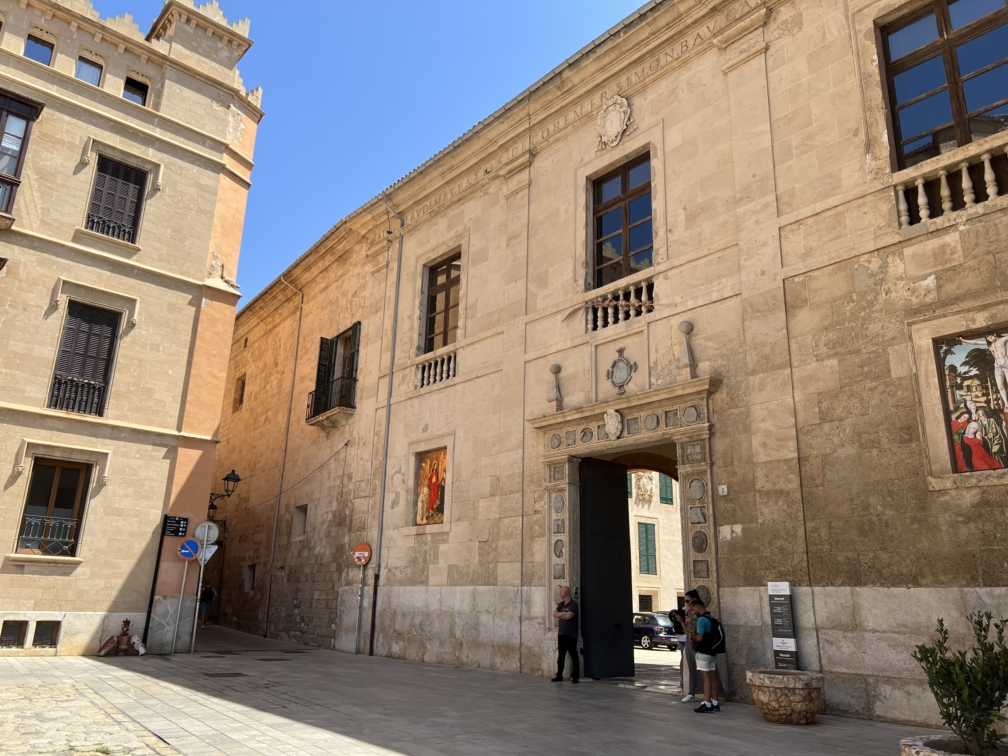
\includegraphics[width=.24\linewidth]{figures/sfm/palma/IMG_1647.jpeg}
} 
\centerline{
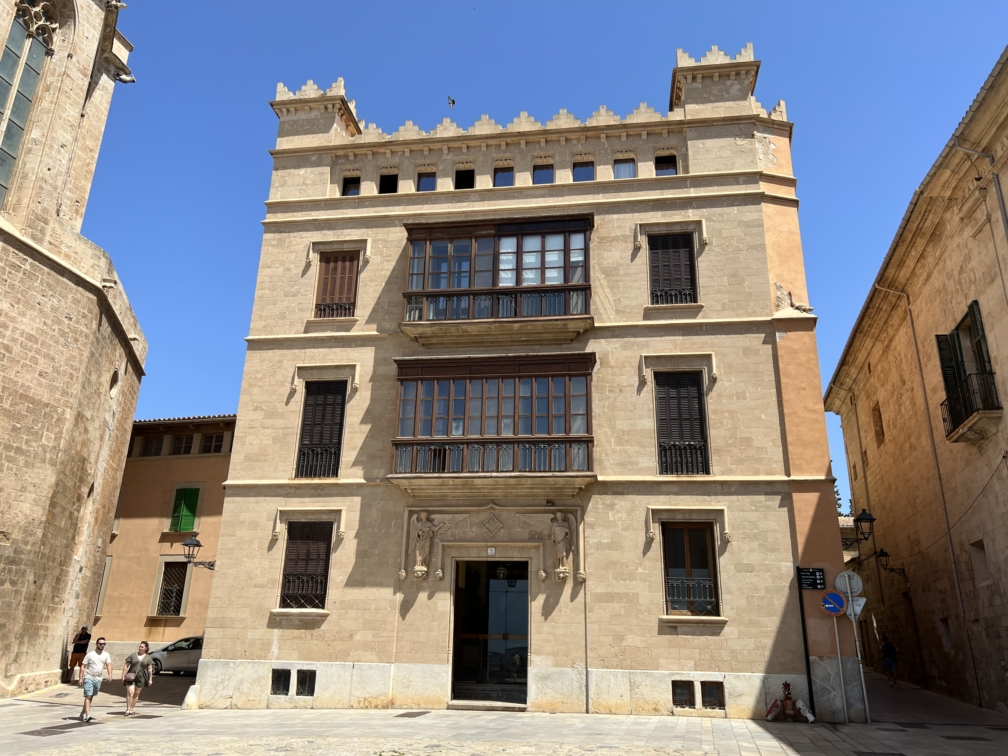
\includegraphics[width=.24\linewidth]{figures/sfm/palma/IMG_1648.jpeg}
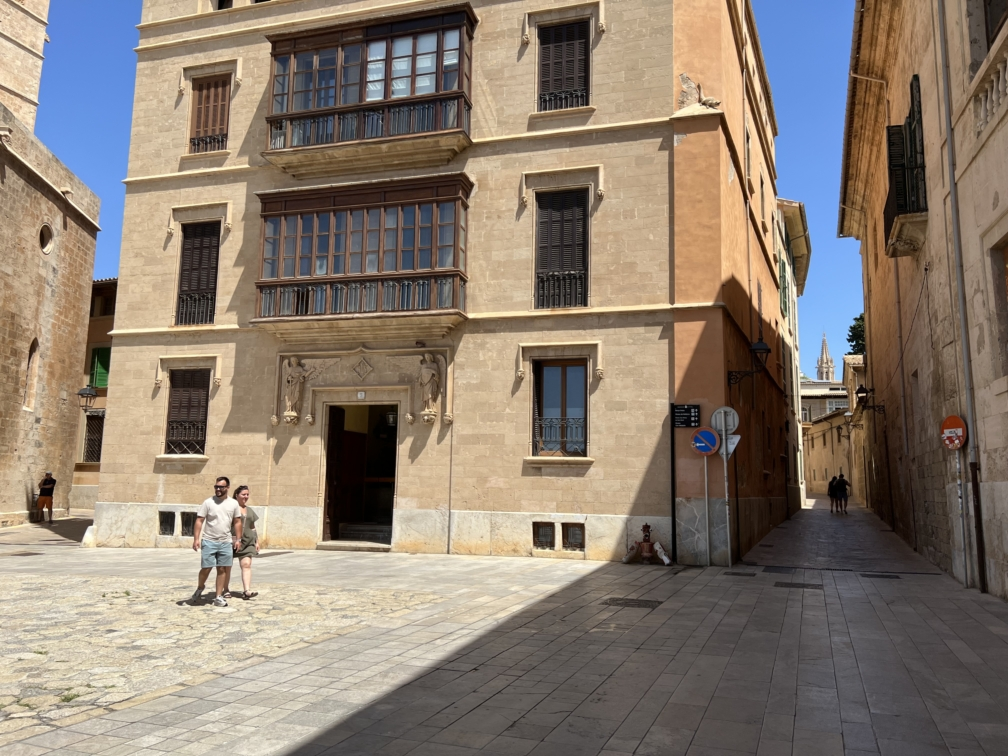
\includegraphics[width=.24\linewidth]{figures/sfm/palma/IMG_1649.jpeg}
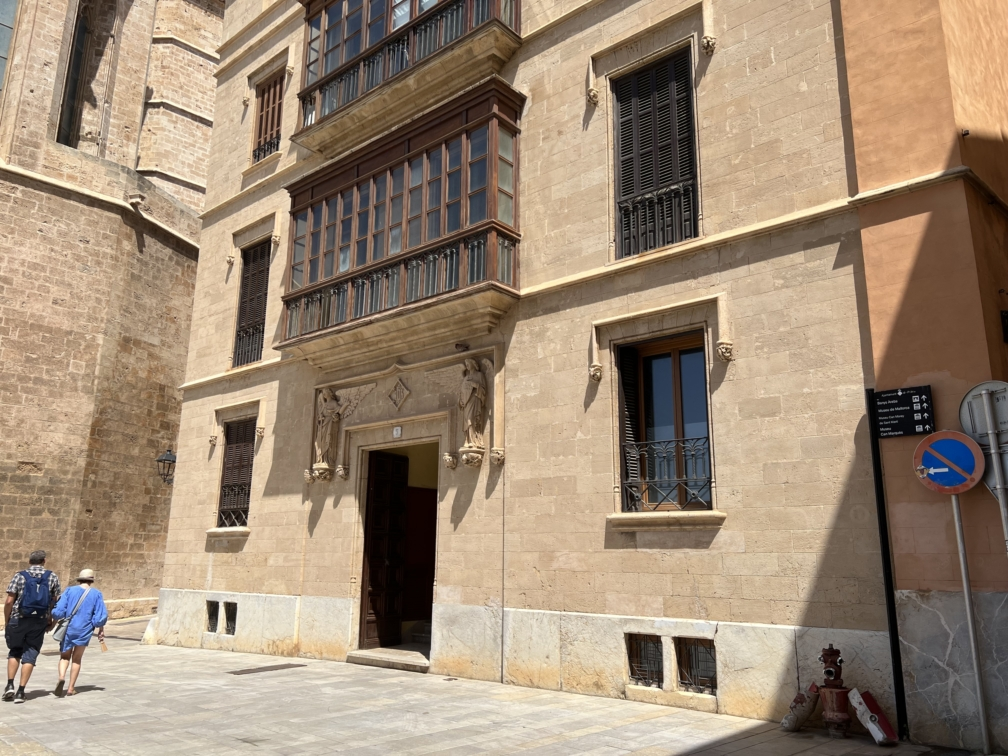
\includegraphics[width=.24\linewidth]{figures/sfm/palma/IMG_1651.jpeg}
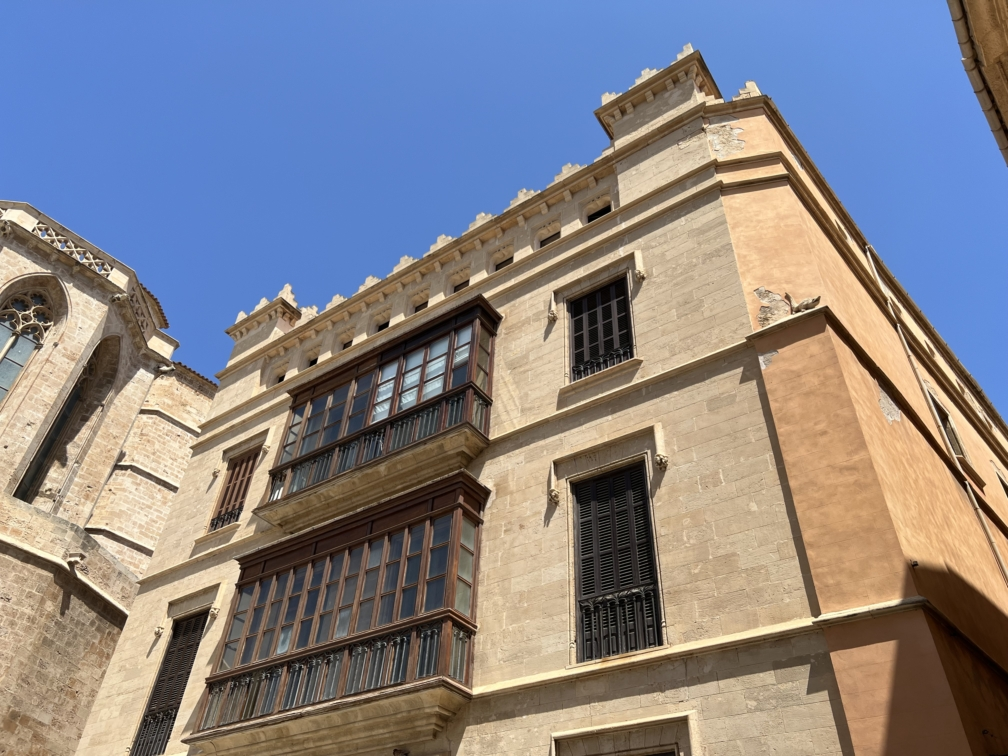
\includegraphics[width=.24\linewidth]{figures/sfm/palma/IMG_1652.jpeg}
} 

\caption{Eight pictures taken in a plaza in Palma de Mallorca, Spain. The images have $3,024 \times 4,032$ pixels.}
\label{fig:sfm:palma}
\end{figure}

%At this point, we admit that we tried the reconstructions of many objects and places, but we were getting only mediocre results before using these images. Sometimes the reconstructions were accurate but hard to understand and, other times the result were just wrong.

\subsection{Problem Formulation}

In the sparse SFM problem, we consider that in the scene there are $N$ distinct points (with $N$ smaller than the number of pixels on each image) that are matched across $M$ different views (we will consider later that not all points may be visible across all images). We denote the $N$ 3D points as $\mathbf{P}_i$.

\marginnote{Notation reminder: we use capital letters for quantities measured in 3D world coordinates and lowercase for image coordinates.}[-.5in] 

For each of the $M$ views (it could be different cameras or different pictures taking by a moving camera), we denote the projection of point $\mathbf{P}_i$ as seen by camera $j$ by $\mathbf{p}^{(j)}_i$. Each view has camera parameters ${\mathbf K}^{(j)}$, ${\mathbf R}^{(j)}$, and ${\mathbf T}^{(j)}$. If all the images are captured by the same camera, then the matrices ${\mathbf K}^{(j)}$ will be the same. In general it is not necessary to make that assumption.  

The goal of the SFM problem is, given the set of corresponding 2D points $\mathbf{p}^{(j)}_i$, recover 3D points $\mathbf{P}_i$, the intrinsic camera parameters, ${\mathbf K}^{(j)}$, and the extrinsic camera parameters ${\mathbf R}^{(j)}$ and ${\mathbf T}^{(j)}$, for each camera $j$.

We will next study what is the minimal number of observations that we need to have any hope of being able to solve the problem. Let's assume that we have calibrated cameras, that is, we know the intrinsic camera parameters for each image, ${\mathbf K}^{(j)}$. We will first count the number of unknowns that we have. We have two sets of unknowns: the 3D coordinates of the $N$ points and the extrinsic camera parameters for the $M$ images.  

This results in 3$N$ unknowns for the $N$ 3D points. For the camera parameters, we assume that the first camera is at the origin. Therefore, we need to figure out the camera matrices for $M-1$ cameras. The rotations can be specified with three numbers, which results in $3(M-1)$ unknowns. The translations (up to a scale factor) result in  $3(M-1)-1$ unknowns. This gives a total of $3N + 6(M-1)-1$ unknowns.

If we have the image coordinates of the $N$ points across the $M$ images, we would have $2NM$ observations (in reality we will have less as some points will only be visible in a subset of the images). So, there is a solution when,
\begin{equation}
2NM \geq 3N + 6(M-1)-1
\end{equation}
Note that if $M=1$, only points captured by one camera are available, then we can not solve the problem. If cameras are uncalibrated, this will add $3M$ additional unknowns (the exact number of additional unknowns will depend on the camera type). 

In the previous description, we are making the assumption that every point is visible in every view (so one can run fundamental matrix estimation, triangulation, and other tasks of each of the $M-1$ cameras with respect to the first view). However, if the visibility criteria isn’t met, for each new image we are adding in to SFM, we will need to triangulate it with respect to its closest image -- when doing so, we may have a slight numerical error, and this new frame may end up having an ever-so-slightly different scale factor with respect to the reconstruction. This accumulates over time, causing {\bf scale drift}.


\subsection{Reprojection Error}

%Explain the reprojection error and make a simple experiment: have one camera and plot the reprojection error as a function of the camera rotation on a semisphere. 

We already introduced the {\bf reprojection error}\index{Reprojection error} in \sect{\ref{sec:cam_cal_minimizing_reprojection_error}} when talking about camera calibration. Here the formulation is similar but we optimize over a different set of unknowns. %Let's write again the reprojection error by let's go step by step this time.  
The reprojection error is the sum of euclidean distances (in heteregenous coordinates) between the observed image points $\mathbf{p}^{(j)}_i$ and the estimated projected points $\hat{\mathbf{p}}^{(j)}_i$
\begin{equation}
\sum_{j=1}^M \sum_{i=1}^N 
\norm{ 
\mathbf{p}^{(j)}_i - \hat{\mathbf{p}}^{(j)}_i 
}
^2 
\end{equation}
The estimated projected points are obtained using the estimated 3D points locations $\mathbf{P}^{(j)}_i$ and the estimated camera matrices $\mathbf{M}^{(j)}$,
\begin{equation}
\sum_{j=1}^M \sum_{i=1}^N 
\norm{ 
\mathbf{p}^{(j)}_i - 
\pi \left( 
\mathbf{M}^{(j)} \mathbf{P}^{(j)}_i 
\right)  
} ^2 
\label{eq:sfm:rep_error}
\end{equation}
where $\pi()$ is the function that transforms a vector described with homogeneous coordinates into the corresponding vector in heterogeneous ones. 

We can make the camera model explicit in \eqn{\ref{eq:sfm:rep_error}} by replacing the camera matrix, $\mathbf{M}^{(j)}$. By using the intrinsic and extrinsic camera matrices we get:
\begin{equation}
\sum_{j=1}^M \sum_{i=1}^N 
\norm{ \mathbf{p}^{(j)}_i - \pi \left( \mathbf{K}^{(j)} 
%\left[\mathbf{R}^{(j)} ~|~ -\mathbf{R}^{(j)}\mathbf{T}^{(j)}  \right]
\begin{bmatrix}
\mathbf{R}^{(j)} ~ \vline ~ -\mathbf{R}^{(j)}\mathbf{T}^{(j)} 
\end{bmatrix}
\mathbf{P}^{(j)}_i \right) 
} ^2 
\end{equation}

To have the final error we still need to add one more factor. We add a {\bf visibility} term, $v_i^{(j)}$, to account for 3D points that are only be visible in a subset of the views.  We will use the binary variable $v_i^{(j)}$ to indicate if point $i$ is seeing from camera $j$. For all the points that are not visible in a view we set $v_i^{(j)}=0$, that is, their reprojection error is ignored. This can be written as:
\begin{equation}
\sum_{j=1}^M \sum_{i=1}^N 
v_i^{(j)}
\norm{ 
\mathbf{p}^{(j)}_i - \pi \left( \mathbf{K}^{(j)} 
%\left[\mathbf{R}^{(j)} ~|~ -\mathbf{R}^{(j)}\mathbf{T}^{(j)}  \right]
\begin{bmatrix}
\mathbf{R}^{(j)} ~ \vline ~ -\mathbf{R}^{(j)}\mathbf{T}^{(j)} 
\end{bmatrix}
\mathbf{P}^{(j)}_i \right) 
} ^2 
\label{eq:final_reprojection_error}
\end{equation}
and this gives us the final reprojection error equation. One common simplification is to assume that all the cameras have the same intrinsic parameters, which means that $\mathbf{K}^{(j)}=\mathbf{K}$. This is the case when the views have been captured by a moving camera with a fixed focal length. The optimization of the reprojection error is also called {\bf bundle adjustment}. 
\index{Bundle adjustment}
\marginnote{The term {\bf bundle adjustment} refers to the process of optimizing the ``bundle of rays'' connecting the camera centers and the coordinates of the 3D points.}


% B. Triggs; P. McLauchlan; R. Hartley; A. Fitzgibbon (1999). "Bundle Adjustment — A Modern Synthesis" (PDF). ICCV '99: Proceedings of the International Workshop on Vision Algorithms. Springer-Verlag. pp. 298–372.



%Before we start to discuss how to minimize the reprojection error, let's look at a few toy problems and study the shape of the error function. 

When optimizing \eqn{\ref{eq:final_reprojection_error}} there are a number of ambiguities that cannot be recovered. Those include a global translation and rotation of the world-coordinate system, the global scale, and a projective ambiguity when $\mathbf{K}$ is unknown. 

%Ambiguities in the recovery. Can we really solve for everything? scale ambiguity, projective ambiguity, ...


There are two main challenges in SFM. The first challenge is that we need reliable matching points, and the second challenge is optimizing \eqn{\ref{eq:final_reprojection_error}}, which is difficult due to local minima and to noisy matches. 


\subsection{Finding Matches across Images}

When describing stereo vision in \chap{\ref{chap:stereo_vision}} we had to find matching points across two views in order to recover depth, but we did not spend much time on the problem of matching points across images. Matching features across views in a stereo pair is challenging, but it is easy in comparison with the challenge of matching points in a multiview setting. Now we will have to match points across views that might be very different, with little overlap and with dramatic camera motions. Therefore, we will need a more robust way to match points. 

%\subsubsection{Detecting Interest Points and Local Descriptors}

%\subsubsection{Finding image features}
\subsubsection{Interest point detector}

The goal of finding image features is to locate image locations that are likely to be stable under different sets of geometric transformations (translation, scaling, rotation, skew, and projective), and illumination changes. These stable regions are called {\bf interest points}. \index{Interest point}
\marginnote{Initially, {\bf interest points} were called {\bf moving elements}. A moving element was any image point that could be identified and followed over time such as a corner, a line termination point, or a texture element \cite{Ullman1979}.}

When talking about stereo matching we described a simple procedure to detect interest points: the Harris corner detector \cite{Harris88}. Corners are examples of image regions that are likely to be distinct from the image surroundings and also be stable under geometric transformations (i.e., corners remain corners under a number of transformations).
There are a number of other important detectors of regions of interest, in addition to the Harris corner detector, such as local extrema of the Laplacian pyramid across space and scale \cite{Mikolajczyk2002,Lowe04}, Harris-Laplace \cite{Mikolajczyk2001}, and maximally stable regions \cite{Matas2004}.  For an in depth description of interest point detectors and their evaluation we refer the reader to the work of Cordelia Schmid et al. \cite{Schmid2000} and Mikolajczyk \cite{Mikolajczyk2002}. 


More recently, the problem of detecting points of interest has been formulated as a learning problem. Given a set of examples of points of interest manually annotated on images, we can train a classifier to automatically label image patches as being centered on a keypoint or not. Some examples of learning-based approaches are Quad-Networks \cite{Savinov2017}, and SuperPoint \cite{DeTone2018}. 


\Fig{\ref{fig:sfm:toy_keypoint_detector}} illustrates a general formulation for detecting keypoints using a classifier. We start by training a classifier using hand-annotated images with keypoints. This can be done by generating simple synthetic images were keypoints are unambiguously defined. The training set can be extended by running an initial keypoint detector on images and then augmenting the images with random geometric transformations. Then we can use the transformed keypoint coordinates together with the transformed images as new ground truth to train a more robust classifier. This is the approach proposed by SuperPoint \cite{DeTone2018}. 


\begin{figure}[t]
\centerline{
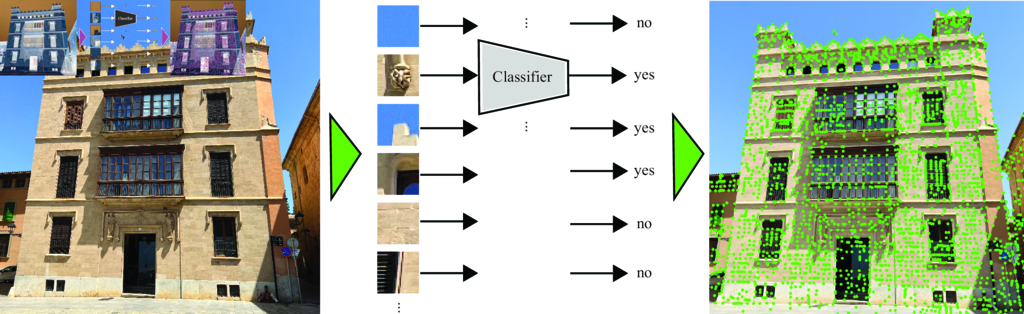
\includegraphics[width=1\linewidth]{figures/sfm/toy_keypoint_detector.eps}
}
\caption{Keypoint detector formulated as a patch classification problem. The classifier labels the patch as containing a keypoint in the center or not.}
\label{fig:sfm:toy_keypoint_detector}
\end{figure}


\begin{figure}[t]
\centerline{
\includegraphics[width=1\linewidth]{figures/sfm/sugar/keypoints_8_3_examples.png}
}
\caption{All the detected keypoints in three views from the sugar bowl. But the images look rather textureless; what is the keypoint detector finding interesting in these images?}
\label{fig:sfm:keypoints_sugar}
\end{figure}

\Fig{\ref{fig:sfm:keypoints_sugar}} shows the resulting detected keypoints by SuperPoint on three viewpoints of the sugar bowl.
The images shown in \fig{\ref{fig:sfm:sugar}} seem to lack texture. Interestingly, when we zoom into the images (which are very high-resolution) we can see that the surface contains many irregularities that are detected by the keypoints classifier (\fig{\ref{fig:sfm:sugar_keypoints_examples_many}}[a]). If the surface of the bowl was smooth and  textureless, the method would fail to detect any interesting points, and the whole pipeline for 3D reconstruction would fail.

The keypoints detected on the plaza scene, shown in \fig{\ref{fig:sfm:sugar_keypoints_examples_many}}{b}, correspond to more obvious keypoints, such as window corners, bricks, and other building details, than the ones detected on the sugar bowl.

\begin{figure}[t]
\sublabel{a}{
\centerline{
\includegraphics[width=1\linewidth]{figures/sfm/sugar/sugar_keypoints_examples_many.eps}
}
}
\sublabel{b}{
\centerline{
\includegraphics[width=1\linewidth]{figures/sfm/palma/palma_keypoints_examples_many.eps}
}
}
\caption{Each patch shows a $65 \times 65$ image crop centered on a detected keypoint. The keypoint detector finds image regions with strong spatial changes. Those regions are also likely to be found on images of the same object but under different viewpoints. (a) Sugar bowl, \fig{\ref{fig:sfm:sugar}}. (b) Plaza, \fig{\ref{fig:sfm:palma}}.}
\label{fig:sfm:sugar_keypoints_examples_many}
\end{figure}






The advantage of hand-engineered detectors is that they are derived from first principles and do not require any training data. However, learning-based detectors can leverage unsupervised learning to achieve state of the art performance. 

%Traditionally, the detection of interest points is performed using a single image.



\subsubsection{Local image descriptors}

Once we have trained a keypoint detector that finds image regions that are distinct and likely to be stable under geometric transformations, we run the detector in the set of images we want to match. We need now to extract at each location a descriptor that will allow finding the same keypoint across the different images. \index{Local image descriptor}

In \chap{\ref{chap:stereo_vision}} we described SIFT  \cite{Lowe04} as a local image descriptor. Other classical descriptors are SURF \cite{Bay2008346}, and ORB \cite{Rublee2011}.
For a review of several hand-engineered descriptors and their evaluation, we refer the reader to the work of Krystian Mikolajczyk and Cordelia Schmid \cite{Mikolajczyk2005}.
% https://www.robots.ox.ac.uk/~vgg/research/affine/det_eval_files/mikolajczyk_pami2004.pdf
\Fig{\ref{fig:sfm:descriptors_sugar}} shows three interest points in the suggar bowl and the three associated descriptors. In this example, each descriptor is a vector of length 256.


\begin{figure}[t]
\centerline{
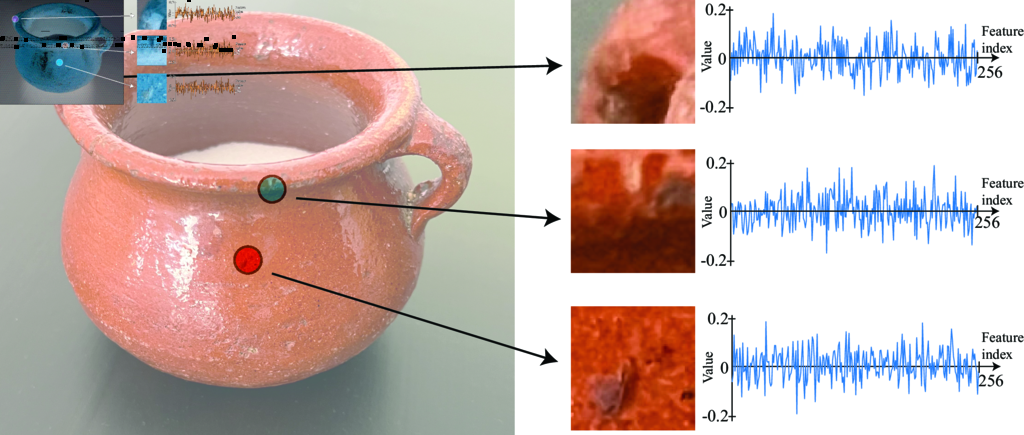
\includegraphics[width=1\linewidth]{figures/sfm/sugar/point_cloud_key_points_figure.eps}
}
\caption{Examples of descriptors for three keypoints. For each keypoint, the figure shows the corresponding image patch and the computed descriptor. Each descriptor has a length of 256 values.}
\label{fig:sfm:descriptors_sugar}
\end{figure}

As shown in \fig{\ref{fig:sfm:palma_keypoint_matching_figure}}, the keypoint detector and descriptor finds image regions and its matches even under different viewpoints and illumination conditions. 
The top row of \fig{\ref{fig:sfm:palma_keypoint_matching_figure}}{a} shows the location of a matching keypoint across six views of the sugar bowl (this keypoint was not detected in the remaining six images). The bottom row shows crops of size $129 \times 129$ pixels around the keypoint. The larger crops allow better getting a sense of the context of each keypoint.
\Fig{\ref{fig:sfm:palma_keypoint_matching_figure}}{b} shows the same for the plaza scene. In this case the keypoint detects the same window corner across multiple views. 


\begin{figure}
\sublabel{a}{
\centerline{
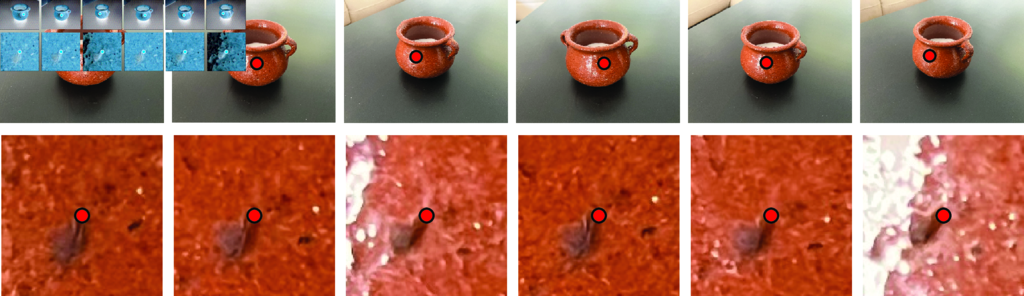
\includegraphics[width=1\linewidth]{figures/sfm/sugar/sugar_keypoint_matching_figure.eps}
}
}
\sublabel{b}{
\centerline{
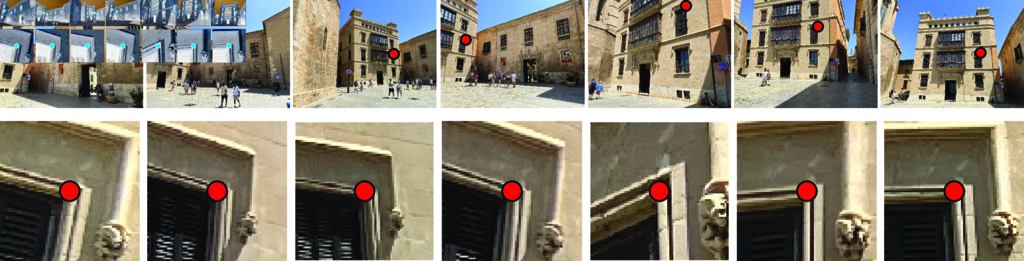
\includegraphics[width=1\linewidth]{figures/sfm/palma/palma_keypoint_matching_figure.eps}
}
}
\caption{Matching keypoints across different viewpoints. For each subfigure, the top row shows the location of a matching keypoint across several views. The bottom row shows crops of size $129 \times 129$ pixels around each the keypoint.}
\label{fig:sfm:palma_keypoint_matching_figure}
\end{figure}




%Classical: SIFT, SURF, ORB
%Learned: SuperPoint, D2-Net

%Image Matching


%We extract SuperPoint features (interest points) and descriptors from each input image. SuperPoint is a lightweight CNN that can run on the CPU if needed -- features extracted from it are often used as drop-in replacements for ORB, SIFT, SURF, etc. (The SuperPoint network is trained in a self-supervised manner, using synthetic datasets created by homography).

We perform brute-force matching, that is, match features from one image with features from every other image because we have a small number of images.
%(but if needed, the hloc library supports a lot of optimization here -- like clustering images by place and only matching among images that are visually similar, etc.). 
For the actual matching shown in this section, we use SuperGlue, another graph network-based matcher. 
%SuperGlue outperforms traditional feature matchers by a significant margin, and is one of the best go-to models that runs on a variety of datasets, without need for fine-tuning.

\subsection{Optimization}

The matching procedure should have given as a set of image points $\mathbf{p}^{(j)}_i$ and visibility indicators $v_i^{(j)}$. Each location will also have a feature, $\mathbf{f}^{(j)}_i$, associated to it. 

There are many different ways in which one can attempt to minimize the loss from \eqn{\ref{eq:final_reprojection_error}}. One standard approach is to do it incrementally starting with only a pair of images. We use the matches between those two images to compute the fundamental and essential matrices, while accounting for outliers using RANSAC. We can then compute an initial 3D reconstruction of the matched points using triangulation as we have already discussed in \chap{\ref{chap:stereo_vision}}. Then, we add another image and we repeat the same process until we have incorporated all the images.  This process will result in a first set of approximated camera poses and 3D locations for a subset of the detected keypoints. 


To find the final set of 3D points,  the camera poses and the 3D locations of the keypoints are then further refined by bundle adjustment (camera intrinsics are refined too, if needed). The reprojection error loss is usually rewritten using a robust cost function (typically the Huber kernel).

Figures \ref{fig:sfm:3dsugar} and \ref{fig:sfm:3dpalma} show the final 3D reconstructions and recovered camera locations for the two sets of images that we have used in this chapter.  


\begin{figure}
\centerline{
\sublabel{a}{
\includegraphics[width=.46\linewidth]{figures/sfm/sugar/point_cloud_sugar_view1.eps}
}
\sublabel{b}{
\includegraphics[width=.46\linewidth]{figures/sfm/sugar/point_cloud_sugar_view2.eps}
} 
}
\caption{3D reconstruction of the sugar bowl. The figure shows two different viewpoints and the recovered camera locations. (a) Bird's view. (b) Side view.}
\label{fig:sfm:3dsugar}
\end{figure}




\begin{figure}
\centerline{
\sublabel{a}{
\includegraphics[width=.46\linewidth]{figures/sfm/palma/3d_palma_view2.eps}
}
\sublabel{b}{
\includegraphics[width=.46\linewidth]{figures/sfm/palma/3d_palma_view1.eps}
} 
}
\caption{3D reconstruction of the plaza. The figure shows two different viewpoints and the recovered camera locations. (a) Bird's view.  (b) Arbitrary view.}
\label{fig:sfm:3dpalma}
\end{figure}



%We take the extracted features and matches, and run COLMAP on them. COLMAP first uses each pair of matched images, computes the fundamental and essential matrices, while accounting for outliers using RANSAC. For every pair of frames, it then computes an initial 3D reconstruction by triangulation. The poses and 3D points are then refined by bundle adjustment (during BA, camera intrinsics are refined too, if needed), using a robust cost function (typically the Huber kernel).


%There aren't many newer SfM references (I usually refer to Bill Triggs' tech report -- I think, from 1998?). There's Chris Sweeney's thesis, which is perhaps the last well-known SfM thesis I've read, but that's at least 7-8 years old

\begin{comment}
\subsection{When it fails}

3D reconstruction using collections of 2D images can be quite reliable if a few conditions are met. But those conditions can fail often. 

As we mentioned in \fig{\ref{fig:sfm:sugar}}, we tried many different scenes before selecting one to show in this book. The reconstruction was successful often, but the results were not illustrative enough, or easy to see when printed and that is the reason why we did not select them. But in some cases, the model just failed in producing the correct results. We will discuss here a couple of examples.

Rubic cube: the model failed to use color properly. All the faces are self similar and without using color cues the image matching procedure cannot reliably tell one face from another. 

Clouds: 

\section{Dense SFM}

While a sparse SFM pipeline results in accurate 3D reconstruction, several applications (such as robotics and computer graphics) require dense 3D scene representations. 

The goal of dense SFM is to reconstruct every pixel from every image, opposed to sparse SFM systems described previously that only reconstruct a subset of pixels.

\end{comment}


SFM is predominantly performed in one of two modes: the incremental mode; and the batch model offline or batch-mode SFM approaches, which compute the scene structure after processing all input images. In this mode, bundle adjustment will only need to be run once, albeit across a potentially large number of cameras and 3D points. This mode allows leverages images from all available viewpoints right from the outset. However, if new images are added the entire SFM pipeline needs to be rerun.

Online, or incremental-mode SFM approaches attempt to estimate scene structure and camera parameters as and when a new image arrives. In this mode, bundle adjustment is run periodically, whenever a sufficient number of points have been newly added. Incremental-mode SFM is often used in applications where all images are not available a priori, or where real-time performance is desired.




\section{Concluding Remarks}

Multiview reconstruction is an active field of research with a wide range of applications in vision, graphics and healthcare. 
While a sparse SFM pipeline results in accurate 3D reconstruction, several applications (such as robotics and computer graphics) require dense 3D scene representations. The goal of dense SFM, not covered here, is to reconstruct every pixel from every image, as opposed to the sparse SFM systems described previously that only reconstruct a subset of pixels.
 
In this chapter, we focused on the most popular variant of SFM used today --- feature-based, or sparse, SFM. In sparse SFM, the 3D reconstruction is computed only for a small subset of the image pixels --- distinct points that may be detected reliably and repeatably across camera pose variations. SFM approaches have also attempted to leverage other kinds of features, such as lines, planes, or objects. Point-based features remain the most popular choice due to their geometric simplicity, and the availability of a wide range of point feature detectors and descriptors.

In dense SFM, the 3D reconstruction is computed for every (or most) of the image pixels. The resulting 3D reconstructions are rich and visually informative, and are useful in applications like robot navigation or mixed reality. Dense SFM approaches usually optimize photometric error, that is, the difference in grayscale or red-green-blue (RGB) intensities of corresponding pixels across images. This is in contrast to the point feature-based methods we looked at in this chapter that minimize a 3D reprojection error. However, these dense SFM techniques tend to be much slower than the sparse SFM methods, and often require more assumptions about the scene or the images, such as the scene being Lambertian (i.e., the grayscale or RGB intensity of a 3D point is invariant to the viewing direction) or the images having a substantially smaller baseline motion compared to the range of motions a point feature-based SFM approach can handle. We will talk about dense optimization of the photometric error when discussing motion estimation in part \ref{part:understanding_motion}.

